
\pagenumbering{roman}

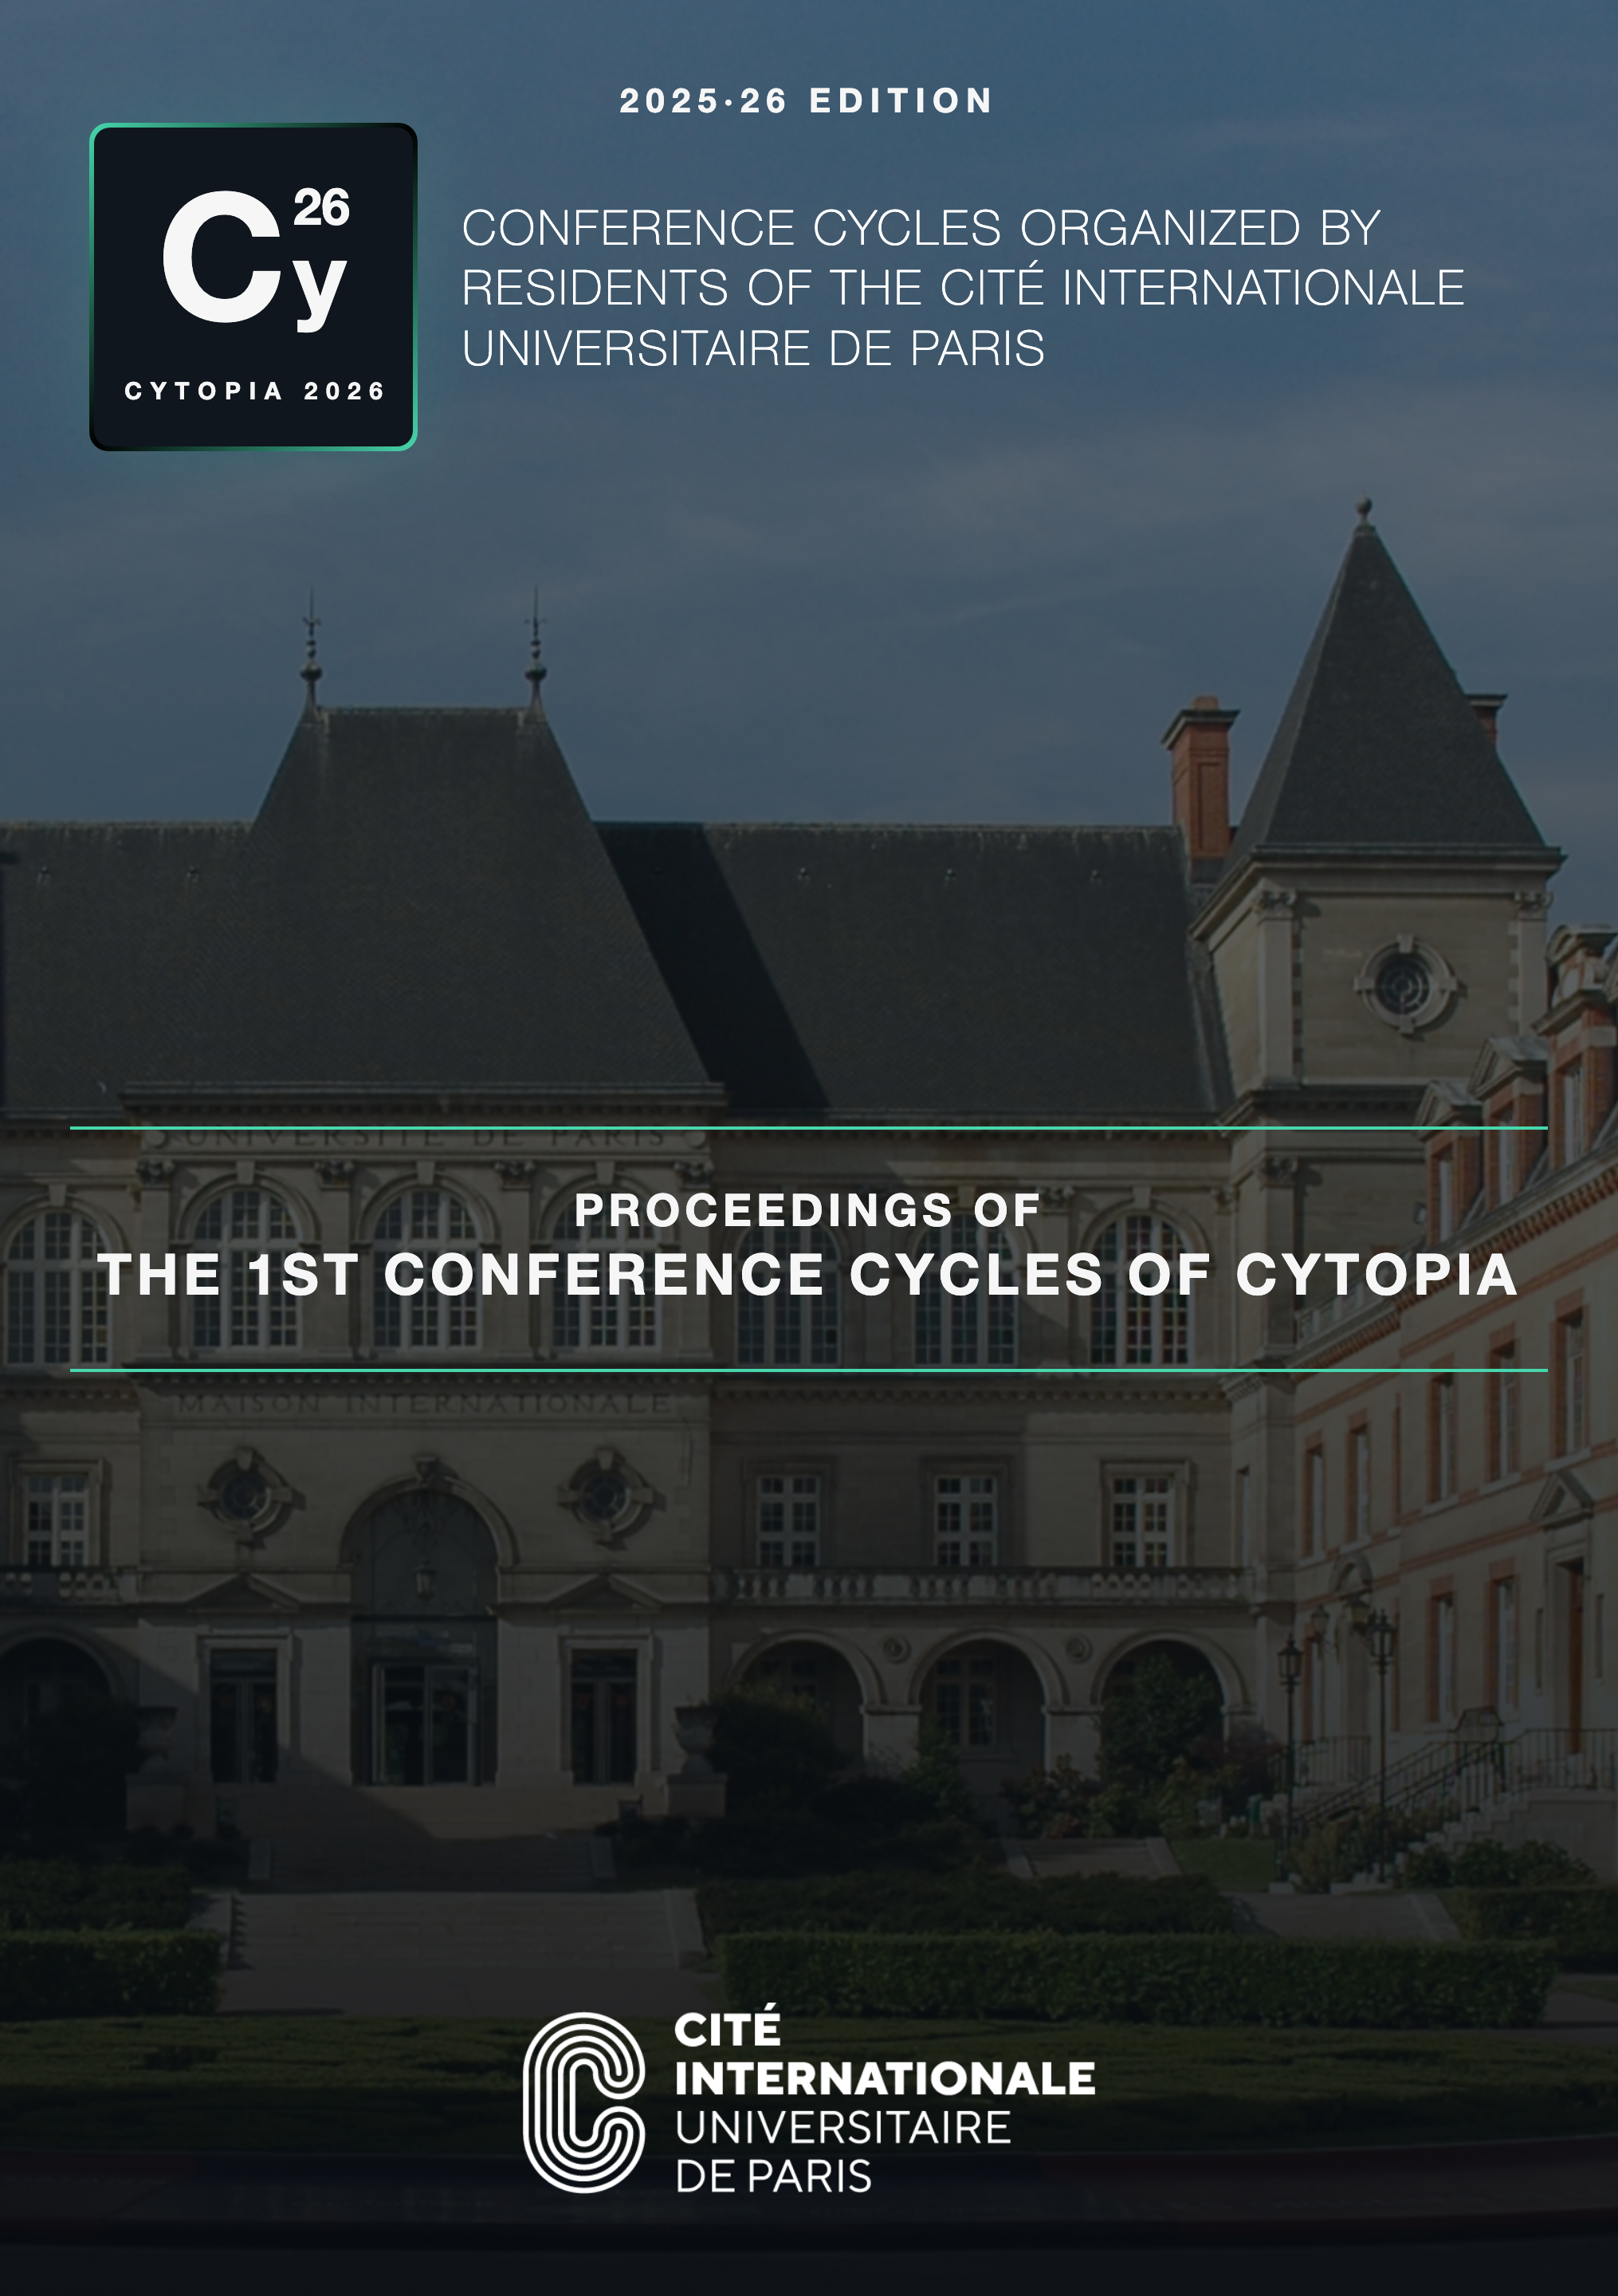
\includepdf[pages=1, scale=1, templatesize={\paperwidth}{\paperheight}, keepaspectratio=false]{fig/cover-book.png}

\cleardoublepage

\null

\cleardoublepage

\chapter*{Preface}\label{preface}
% \addcontentsline{toc}{chapter}{Preface}

\markboth{Preface}{Preface}

\emph{Cytopia} is a series of conference cycles held at the \emph{Cité
internationale universitaire de Paris} (\texttt{CiuP}). Each cycle
brings together abstracts, articles, and presentations centered on a
shared theme, while creating an interdisciplinary space that combines
reflection, debate, and knowledge production.

What began as a single series focusing on emerging \emph{technologies}
has been expanded to include two other major themes: \emph{diplomacy}
and \emph{biology}, proposed by two other \texttt{CiuP} associations:
\emph{DiploCité} and \emph{Gene \& Tonic}.

For this first edition of the \emph{Cytopia} multi-cycle conferences, we
are pleased to feature these three themes, which offer rich
content---not only through the live presentations they inspired but also
through the editorial content presented in this volume, which compiles
the conference proceedings. Looking ahead, \emph{Cytopia} could expand
to include as many series as there are themes within a campus as
culturally, artistically, and academically rich as the \texttt{CiuP}.

The format of \emph{Cytopia} conferences lies at the intersection of the
dynamics of an open and international campus, a conference/workshop
where ideas and knowledge are shared in various formats: discussions,
abstracts, articles, and presentations.

This hybrid approach allows for the introduction of innovative tools
that differ from traditional conference models. Each of the formats
described above is indexed so that they can be accessed by
conversational agents (powered by artificial intelligence). Each text
presented in this book includes a \emph{QR code} that allows readers to
initiate a conversation with the text to better understand it and access
certain nuances discussed in previous presentations and interviews.

\emph{Cytopia}, \emph{DiploCité}, and \emph{Gene \& Tonic}\footnote{Here,
  and throughout the book, we follow the timeline or the alphabetical
  order of group/cycle names to establish the sequence in which they
  appear in this volume.} hope you enjoy reading and discussing this
format, inspired by the first \emph{Cytopia} conference proceedings
presented at the \texttt{CiuP}.

\begin{quote}
\emph{Hugues Wattez}
\end{quote}

\newpage

\null

\cleardoublepage